\begin{tikzpicture}[remember picture, overlay]
  \node[
    fill=orange!70!black,                 % Цвет заливки
    opacity=0.6,                 % Прозрачность
    minimum width=0.9\paperwidth,  % Ширина = 90% ширины страницы
    minimum height=0.08\paperheight, % Высота = 8% высоты страницы
    anchor=north east            % ЯКОРЬ Прямоугольник привязан за свой ВП угол
  ] 
  at (current page.north east)     % ПОЗИЦИЯ Якорь помещается в ВП угол страницы
  {};

  \node[
    text=white,
    anchor=center,
    yshift=-0.065\paperheight
  ] 
  at (current page.north)
  {
    \normalsize\bfseries СОБЕРИ КВАДРАТ
  };

  \node[
    text=white,
    anchor=north east,
    yshift=-0.053\paperheight,
    xshift=-0.065\paperwidth
  ] 
  at (current page.north east)
  {
    \Large\bfseries 9
  };
  
\end{tikzpicture}

\begin{tikzpicture}[remember picture, overlay]
  \node[
    fill=orange!70!black,
    opacity=0.6,
    minimum width=0.07\paperwidth,
    minimum height=0.08\paperheight,
    anchor=south east
  ] 
  at (current page.south east)
  {};
\end{tikzpicture}


\begin{tikzpicture}[remember picture, overlay]
  \node[anchor=north west, 
        xshift=0.14\paperwidth,
        yshift=-0.09\paperheight]
        at (current page.north west) 
  {
    \begin{minipage}{0.5\textwidth}
      \raggedright
      \textbf{\textsl{Словарик}}
      \vspace{2mm}
      
      % Таблица
      \begin{tabular}{|l|c|}
        \hline
        Разрезание большого прямоугольника на маленькие & Электрическая цепь \\
        \hline
        Вертикальный разрез & Узел \\
        \hline
        Маленький прямоугольник & Резистор \\
        \hline
        Длина его вертикальной стороны & Сила тока через резистор \\
        \hline
        Отношение его горизонтальной стороны к вертикальной & Сопротивление резистора \\
        \hline
        Вертикальный стороны большого прямоугольника & Клеммы батарейки \\
        \hline
        Длина его вертикальной стороны & Сила тока через батарейку \\
        \hline
        Длина его горизонтальной стороны & Напряжение батарейки \\
        \hline
        Отношение его горизонтальной стороны к вертикальной & Сопротивление электрической цепи \\
        \hline
      \end{tabular}
    \end{minipage}
  };
\end{tikzpicture}

\begin{textblock*}{0.82\paperwidth}(0.08\paperheight, 0.35\paperwidth)
    \begin{multicols}{2}
    {
    \justifying
    \textbf{Теорема.} \textit{Пусть квадрат разрезан на прямоугольники с отношением сторон $r$. Тогда $r$ – корень ненулевого многочлена с целыми коэффициентами.} \par \textbf{Доказательство.} Применим такой трюк: растянем квадрат в $r$ раз по горизонтали. Получим прямоугольник с отношением сторон $r$, разрезанный на квадраты и прямоугольники с отношением сторон $r^2$. Сопоставим разрезанию электрическую цепь. Она состоит из резисторов сопротивлением 1 и $r^2$, а сама имеет сопротивление $r$. По лемме о сопротивлении цепи, число $r$ можно выразить через числа 1 и $r^2$ с помощью четырех арифметических действий. Значит, найдутся два ненулевых многочлена $p(x)$ и $q(x)$ с целыми коэффициентами, такие, что $r$ = $\frac{p(r^2)}{q(r^2)}$, т.е. $q(r^2) \cdot r - p(r^2) = 0$. Получили, что $r$ – корень многочлена $q(x^2) \cdot x - p(x^2)$ - с целыми коэффициентами. Этот многочлен не равен тождественно нулю, так как многочлены $p(x^2)$ и $q(x^2)$ – ненулевые, причем $x$ входит в многочлен $q(x^2) \cdot x$ только в нечетной степени, а в многочлен $p(x^2)$ – только в четной. Теорема доказана. \par В обратную сторону теорема неверна. Например, квадрат нельзя разрезать на прямоугольники с отношением сторон $\sqrt{2}$ (докажите!), хотя это число – корень многочлена $x^2 - 2$. \par \centerline{\textbf{Разрезания для $\mathbf{r}$ вида $\mathbf{a} + \mathbf{b}\sqrt{2}$}} Попробуем найти все числа $r$ вида $a + b\sqrt{2}$ , где $a$ и $b$ – рациональны, для которых квадрат разрезается на прямоугольники с отношением сторон $r$. Числа вида $r = a + b\sqrt{2}$ с рациональными $a$ и $b$ мы будем называть \textit{хорошими}. Число $\overline{r} = a - b\sqrt{2}$ назовем \textit{сопряженным} к хорошему числу $r = a + b\sqrt{2}$. Сопряженное число определено однозначно, потому что хорошее число единственным образом представляется в виде $r = a + b\sqrt{2}$ с рациональными $a$ и $b$ (проверьте!). \par \textbf{Лемма об операциях над хорошими числами.} \textit{Если $x$ и $y \neq 0$ – хорошие, то и $x + y$, $x - y$, $x \cdot y$, $x/y$ – хорошие, причем $\overline{x + y} = \overline{x} + \overline{y}$, $\overline{x - y} = \overline{x} - \overline{y}$, $\overline{x \cdot y} = \overline{x} \cdot \overline{y}$}, $\overline{x/y} = \overline{x}/\overline{y}$. \par \textbf{Доказательство.} Пусть $x = a + b\sqrt{2}$, $y = c + d\sqrt{2}$, где $a, b, c, d$ рациональны. Тогда сразу видим, что \par \centerline{$x + y = (a + c) + (b + d)\sqrt{2}$,} \par \centerline{$x - y = (a - c) + (b - d)\sqrt{2}$,} \par \centerline{$x \cdot y = (ac + 2bd) + (ad + bc)\sqrt{2}$} \par - хорошие. Для частного $x/y$ нужно ещё применить обычный прием - «домножить на сопряженное»: \par 
    \begin{multline*}
    \frac{x}{y}=\frac{a + b\sqrt{2}}{c + d\sqrt{2}}=\frac{(a + b\sqrt{2})(c - d\sqrt{2})}{(c + d\sqrt{2})(c - d\sqrt{2})}= \\
    = \left(\frac{ac - 2bd}{c^2 - 2d^2}\right) + \left(\frac{bc - ad}{c^2 - 2d^2}\right)\sqrt{2}.
    \end{multline*}
    Видим, что и оно - хорошее ($c^2 - 2d^2$ не равно нулю, так как $y$ не равно нулю). Так же легко вычисляются сопряженные, например, \par
    \begin{multline*}
    \overline{x \cdot y}=(ac + 2bd) - (ad + bc)\sqrt{2}= \\ 
    = (a - b\sqrt{2})(c - d\sqrt{2}) = \overline{x} \cdot \overline{y}.
    \end{multline*}
    Лемма доказана. \par {\small\textbf{Задача 5.} Можно ли представить $1 + \sqrt{2}$ в виде суммы квадратов нескольких хороших чисел?} \par
    \begin{multicols}{2}
    Приведем пример разрезания квадрата на прямоугольники с отношением сторон $r = a + b\sqrt{2}$ в случае, когда сопряженное к нему положительно. Возьмем прямоугольник со сторонами 1 и $a + b\sqrt{2}$. Назовем его \textit{эталонным}. Умножим стороны эталонного прямоугольника на число $\overline{r}$. Получим прямоугольник со сторонами $a - b\sqrt{2}$ и $a^2 - 2b^2$, и он подобен эталонному. Запишем $a^2-2b^2$ в виде $k/l$ для
    \begin{figure}[h]
    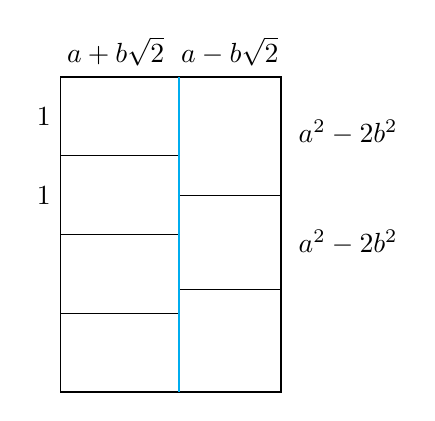
\begin{tikzpicture}
    \draw (0,1) rectangle (1.5,0);
    \draw (0,2) rectangle (1.5,1);
    \draw (0,3) rectangle (1.5,2);
    \draw (0,4) rectangle (1.5,3);
    \draw (1.5,2.5) rectangle (2.8, 4);
    \draw (1.5,1.3) rectangle (2.8, 2.5);
    \draw (1.5,0) rectangle (2.8, 1.3);
    \draw[cyan, thick] (1.5,0) -- (1.5,4);
 
    \node[above] at (0.7,4.02) {$a+b\sqrt{2}$};
    \node[above] at (2.15,4.02) {$a-b\sqrt{2}$};
    \node[right] at (2.9,3.3) {$a^2-2b^2$};
    \node[right] at (2.9,1.9) {$a^2-2b^2$};
    \node[left] at (0,2.5) {1};
    \node[left] at (0,3.5) {1};
    \end{tikzpicture} 
    \caption*{\textsl{Рис. 12. Вот так из прямоугольников с хорошим отношением сторон можно составить прямоугольник с рациональными сторонами}}
    \end{figure}
    \end{multicols}
    }
    \end{multicols}
\end{textblock*}
